\documentclass[main.tex]{subfiles}
\begin{document}

\chapter{Appendix}
\section{Bloch Sphere Visualization}%
\label{sec:bloch-sphere}
\begin{figure}[H]
    \centering
    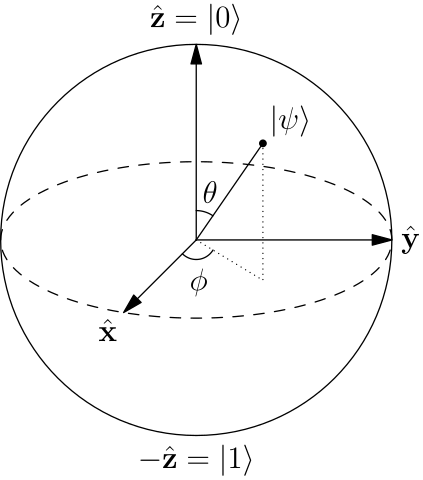
\includegraphics[width=0.3\textwidth]{figs/bloch_sphere.png}
    \caption{Representation of an abritrary pure quantum state on the Bloch sphere.
    \\ Source:~\cite{glosser.ca_english:_2012} (CC BY-SA 3.0).
    }%
    \label{fig:bloch_sphere}
\end{figure}

The pure state of a qubit can be visualized on the surface of a unit sphere with the following parametrization
\begin{equation}
    \ket{\psi} = \cos(\frac{\theta}{2})\ket{0} + \ex^{i\phi}\sin(\frac{\theta}{2})\ket{1}
\end{equation}
where \( \theta \) and \( \phi \) are the angles shown in \Cref{fig:bloch_sphere}.
The ground state \(\ket{0}\) is located on the ``north pole'' and the excited state \(\ket{1}\) on the ``south pole''.

Further, a handy trick to visualize the qubit when it has more than two levels is to ``project'' the state to the \(\qty{\ket{0},\ket{1}}\) basis with \( \op{0} + \op{1} \) and then plot it on the Bloch sphere.
This means that the subspace which is not spanned by the first two levels will be represented by the inside of the sphere.
For example, the state \(\ket{2}\) will lie right in the center of the sphere while \(\qty(\ket{1}+\ket{2})/\sqrt{2}\) will lie halfway between the center and the south pole.

%\subsection{Wigner function}
%The wigner function can be used to visualize quantum states and processes.
%It is a quasiprobability distribution where states exhibiting quantum phenomena will have negative values, impossible for classical states.

% TODO Explain why the wigner function is good for visualization.

\newpage
\section{Cat Code Supplementary Figures}
\subsection{Wigner Function of Resonator Target States}%
\label{sec:resonator-target-wigner}
The six target states in the cat code basis are shown in \Cref{fig:cat-resonator-wigner-targets} with \(\alpha=2\) and a Hilbert space trunacted at a size of \(N_r=8\).
Looking at the Wigner function of \(\ket{0}\) in (the logical cat code basis), we can see two lobes with an interference fringe in between them.
For large enough \(N_r\) the lobes will appear circular.
Compared to the basis states, the superposition states exhibit even more complex shapes.

\begin{figure}[ht]
	\centering
	\foreach \n/\capn [count=\ni] in {{0}/{\ket{0}},{5}/{\ket{1}},{3}/{(\ket{0}+\ket{1})/\sqrt{2}},{1}/{(\ket{0}-\ket{1})/\sqrt{2}},{2}/{(\ket{0}+i\ket{1})/\sqrt{2}},{4}/{(\ket{0}-i\ket{1})/\sqrt{2}}}{
		\subcaptionbox{\(\capn{}\)}{
			\centering
			\includegraphics[width=0.30\textwidth]{figs/cat_wigner_targets_\n.png}
		}%
		\ifnum\ni=6%
				%
		\else%
			\hfill
		\fi%
	}
	\caption{%
	Wigner function of the six target states in the cat code basis with \(\alpha = 2\) and \(N_r=8\).
	}%
	\label{fig:cat-resonator-wigner-targets}
\end{figure}

\subsection{Occupation Dynamics of Resonator During State Transfer}%
\label{sec:resonator-occupation}
The occupation dynamics for the resonator during the state transfer are plotted in \Cref{fig:cat-resonator-occupation}.
\begin{figure}[H]
	\centering
	\foreach \n/\capn [count=\ni] in {{0}/{\ket{0}},{5}/{\ket{1}},{3}/{(\ket{0}+\ket{1})/\sqrt{2}}}{
		\subcaptionbox{Transfer of \(\capn{}\)}{
			\centering
			\setlength\figureheight{20em}
			\setlength\figurewidth{\textwidth}
			\input{figs/cat_res_occ_60,0_\n.tikz}
		}%
		\ifnum\ni=3%
				%
		\else%
			\hfill
		\fi%
	}
	\caption{Resonator level occupation over time for the six state transfers.}%
\end{figure}
\begin{figure}[H]\ContinuedFloat{}
	\centering
	\foreach \n/\capn [count=\ni] in {{1}/{(\ket{0}-\ket{1})/\sqrt{2}},{2}/{(\ket{0}+i\ket{1})/\sqrt{2}},{4}/{(\ket{0}-i\ket{1})/\sqrt{2}}}{
		\subcaptionbox{Transfer of \(\capn{}\)}{
			\centering
			\setlength\figureheight{20em}
			\setlength\figurewidth{\textwidth}
			\input{figs/cat_res_occ_60,0_\n.tikz}
		}%
		\ifnum\ni=3%
				%
		\else%
			\hfill
		\fi%
	}
	\caption{Resonator level occupation over time for the six state transfers.}%
	\label{fig:cat-resonator-occupation}
\end{figure}

\newpage
\section{Jupyter Notebooks and Optimization Data}
\label{sec:jupyter}
To ease the reproducibility of the simulations the Jupyter notebooks used in this thesis and majority of resulting data are available at \url{https://github.com/JohanWinther/cat-state-encoding}.
Even though the code isn't provided in a structured fashion it will still be provided publicly so as to encourage code and data sharing.

\end{document}
